\chapter{Implémentation}
	\section{Introduction}
	
	Notre projet s'intègrent dans un projet de recherche scientifique. De ce fait, une implémentation efficace et optimisée de notre conception est nécessaire. Nous commencerons ce chapitre par présenter l'architecture existante et comment nous l'avons étendue avec nos deux moteurs tout en détaillant les différentes couches de cette architecture. Nous conclurons par présenter l'environnement de développement.
	
	
	\section{Architecture globale}
	
	L'architecture existante est une architecture en pipeline de 3-tiers. Nous utiliserons cette architecture pour le backend de la solution. Elle se compose de trois couches logicielles que nous avons enrichies avec nos deux moteurs. Nous les présenterons ci-dessous:
	
	\begin{enumerate}
	\item \textbf{La couche données ou persistance :} cette couche est responsable de la gestion des données en entrée et les fonctions d'accès et de stockage. Les données en entrées ainsi que les résultats de compression sont sous forme de fichiers.
	
	\item \textbf{La couche traitement :} c'est le noyau des moteur de compression de notre projet. Elle inclue tout les algorithmes de compression et de manipulation des graphes. 
	
	\item \textbf{La couche présentation :}  Deux types de résultats (fichiers) sont produits : le premier est le graphe compressé, le deuxième représente le fichier log des performances. 
	\end{enumerate}
		
	
\begin{figure}[H]
	\centering
	\label{Img:archglob}
	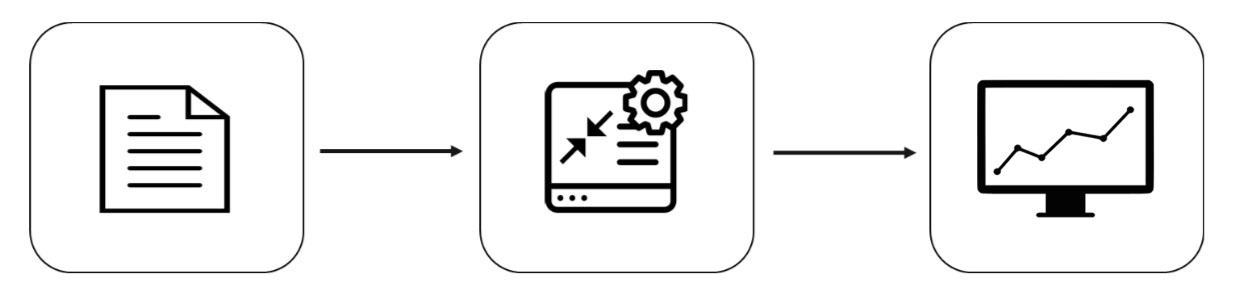
\includegraphics[scale=0.35]{ressources/image/ArchGlob.jpg}
	\caption{Architecture du backend}

 \end{figure}
	
	Dans le but de faciliter l'exploitation et l'utilisation de notre solution, nous proposons une application web qui permettra  d'accéder au différentes fonctionnalités offertes. Cette proposition se base sur le fait que les performances des machines ordinaires s'avèrent limiter pour l'exécution des algorithmes de compression dans le cas des grands graphes. L'utilisation d'un serveur web performant nous semble la solution la plus adéquate. La figure \ref{Img:archglob2} montre l'architecture globale de la solution.   	
	
\begin{figure}[H]
	\centering
	\label{Img:archglob2}
	
\includegraphics[scale=0.35]{ressources/image/ArchGlob2.jpg}
	\caption{Architecture globale de la solution web}
 \end{figure}
 
 Dans ce qui suit, nous détaillerons uniquement les couches de l'architecture du backend ainsi que les bibliothèques qui les constituent. Les détails des autres couches de l'architecture globale ne seront pas présenter car elles n'influence en aucun cas sur les résultats de compression. Elle permettent uniquement d'offrir une interface ergonomique et une exécution distante tirant profit des performances du serveur utilisé.
	
	\section{Données}
	Les données manipulées par les moteurs de compression sont tous sous format de fichiers textes. La structure de ses fichiers diffère selon le type de graphe en entrée. Comme nous l'avons déjà implicitement mentionnées, l'implémentation proposée prend en charge les types de graphes suivants : graphe dynamique orienté, graphe statique (orienté et non orienté) et finalement graphe étiqueté. Nous présenterons dans ce qui suit leurs structures:
	
	\begin{itemize}[label=$\bullet$]
	\item \textbf{Graphe statique:}
	
	\begin{figure}[H]
	\centering
	\label{Img:statiqugr}
	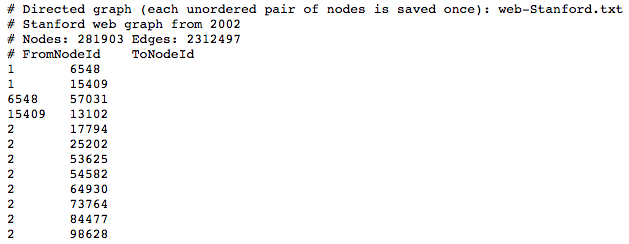
\includegraphics[scale=0.65]{ressources/image/statiqugr.png}
	\caption{Structure d'un fichier de graphe statique}
 \end{figure}
	
	Le fichier représentant un graphe statique est composé de plusieurs lignes chacune faisant référence à un des liens du graphe de données. Elles incluent l'identifiant de la source suivi de  l'identifiant de la destination. Les lignes dont le premier caractère est un "\#" sont ignorées.
	\item \textbf{Graphe dynamique: } 
	
	\begin{figure}[H]
	
	\label{Img:dynamiqgr}
	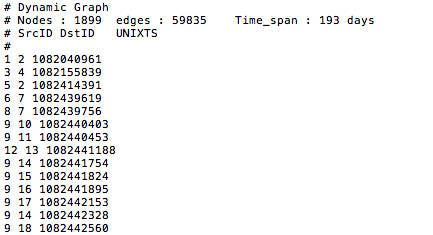
\includegraphics[scale=0.7]{ressources/image/dynamiqgr.png}
	\caption{Structure d'un fichier de graphe dynamique}
 \end{figure}
Les liens dans un graphe dynamique sont représentés par trois composantes (u,v,t)	signifiant qu'un lien entre les nœuds u et v est apparu à l'instant t. Chaque lien représente une ligne dans le fichier de données.
	
	\item \textbf{Graphe étiqueté:} 
	\begin{figure}[H]
	
	\label{Img:etiqGr}
	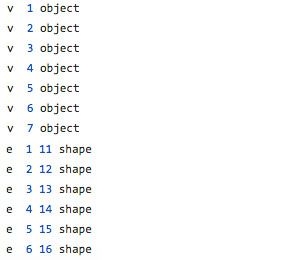
\includegraphics[scale=0.6]{ressources/image/etiquegr.png}
	\caption{Structure d'un fichier de graphe étiqueté}
 \end{figure}

Le fichier de données d'un graphe étiqueté est composé de deux types de lignes: les lignes commençant avec un "$v$" représentent les identifiants des sommets suivis de leurs étiquettes et les lignes commençant avec un "$e$" représentent les identifiants des liens suivis de leurs étiquettes.
	
	\end{itemize}
	
	
	
	\section{Traitement}

Dans cette section, nous détaillerons les principales structures utilisées pour représenter les graphes en mémoire ainsi que les fonctions et méthodes décrivant les interfaces de nos deux moteurs compression. 
\subsection{Les structures utilisées }
Nous nous intéressons dans notre projet à trouver un bon compromis entre les performances de la compression (taux de compression et le nombre de bits par lien) et le temps d'exécution. Pour cela nous avons essayer de choisir des implémentations de structures de données qui répondent à cette contrainte.

\begin{enumerate}[label=(\alph*)]
\item \textbf{TNGraph :}
Cette structure est l'une des structures les plus performantes offertes par la bibliothèque \newacronym{snap}{SNAP}{Stanford Network Analysis Package}	 \gls{snap} (voir section \ref{snaplib}). Elle représente un graphe orienté et est implémenté à l'aide de fonctions de hachages offrant ainsi un temps d'accès très rapide. Elle offre aussi une panoplies d'opérations facilitant la manipulation du graphe de données.

\item\textbf{TUNGraph :}
Cette structure est aussi une des structures de la bibliothèque \gls{snap}. Elle représente un graphe non orienté et offre les mêmes avantages que la structure précédente. 

\item\textbf{std::vector<Boost::dynamicbitset<> > :}
 Nous avons adopté cette structure pour représenter la matrice d'adjacence en mémoire. Les lignes de la matrice d'adjacence sont représentées par un vecteur de bits de la bibliothèque Boost donnant un accès rapide parmi toutes les implémentation disponibles  \citep{pieterse2010performance}. Les tableaux de lignes seront stockés dans un tableau dynamique de la bibliothèque standard du langage c++ permettant d'exploiter la localité du cache vu que ses éléments sont stockés de façon contigüe en mémoire.
 
\item\textbf{std::vector<std::pair<std::vector<unsigned int>,unsigned int> >:}
Cette structure représente la liste d'adjacence d'un graphe. Comme nous l'avons déjà expliquer nous dotons chacune des listes par un pointeurs indiquant la position du dernier élément visité. Les paires ( listes, pointeurs ) seront stockées dans un tableau indexé par les identifiants des nœuds du graphes ( 0...N ).

\item\textbf{LabeledGraph :} Pour les graphes étiquetés, nous proposons d'utiliser notre propre structure intitulée << \textit{LabeledGraph} >>.

\item \textbf{std::map<unsigned int,TNGraph> :}
La dernière structure sont les graphes dynamiques orientés qui sont représentés par les paires ($t_i$ , $G_i$) où $G_i$ représente une capture du graphe de données à l'instant $t_i$.


\end{enumerate}



\subsection{Les méthodes et fonctions }
	Nous présenterons ci-dessous les principales fonctions et méthodes décrivant le schéma globale de fonctionnement de nos deux moteurs.
	
	\begin{enumerate}[label=(\alph*)]
		\item \textbf{LoadGraph :} Cette fonction permet de charger le graphe de données en mémoire à partir d'un fichier texte. Elle prend en paramètres le fichier de données ainsi que le type de graphe dans le cas du moteur P-GraCE. Tant dis que dans le cas du moteur $k^2$-GraCE, elle prend en paramètres le fichier de données, le type de graphe ainsi que le type représentation à utiliser pour compresser le graphe.
		\item \textbf{CompressK2 :} Cette fonction consiste en le processus de compression du graphe en utilisant les arbres $k^2$-trees. Elle reçois en entrée le graphe de données et son type et donne en sortie les deux listes T et L représentant l'arbre $k^2$-trees.
		
		\item \textbf{CompressPattern :} Cette fonction permet de compresser le graphe de données en utilisant ses sous-structures les plus importantes. Elle prend en paramètres le graphe de données ainsi que le choix de la méthode d'extraction de motifs à utiliser dans le processus de compression.
		
		\item \textbf{SaveCompressed :}  Cette fonction effectue la sauvegarde du résultat de compression dans un fichier texte.
		
	\end{enumerate}	
	
	Le schéma de la figure \ref{Img:functMethod} montre le schéma globale de fonctionnement des deux moteurs:  
	
	\begin{figure}[H]
	
	\label{Img:functMethod}
	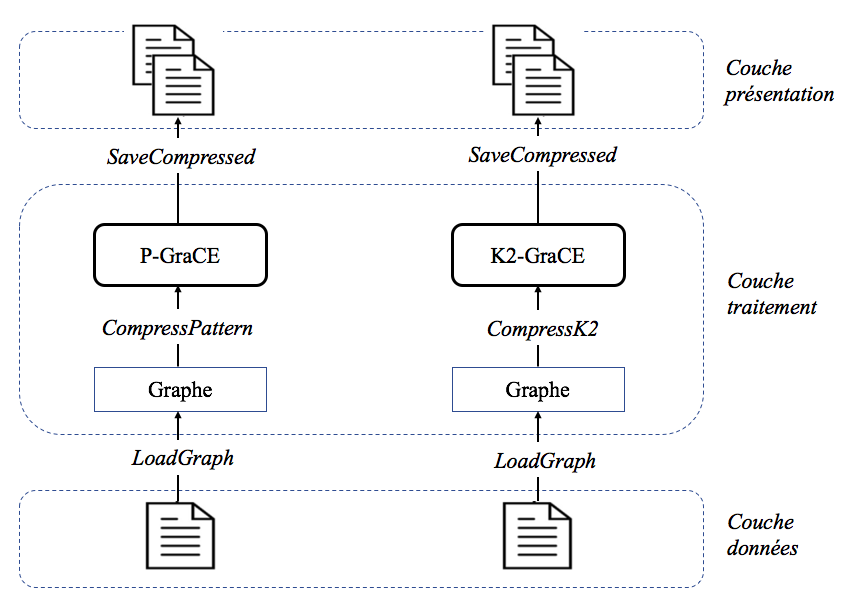
\includegraphics[scale=0.5]{ressources/image/funct.png}
	\centering
	\caption{Schéma globale du fonctionnement des deux moteurs}
 \end{figure}
	
	
	\section{Présentation}
	
	La couche présentation est responsable de donner accès à toutes les fonctionnalités offertes par notre solution, entre autres le choix des paramètres pour différentes méthodes, ainsi que de visualiser les résultats. En plus du fichier de sortie, elle fournit les différentes mesures de performances. Elle offre ainsi aux chercheurs la possibilité de comparer les performances de différents méthodes sur un même graphe. 
	
	\section{Environnement de développement}
		
		Le choix des outils de développement dans tout projet informatique est très important vue leur fort impact sur les performances du produit finale. Comme notre solution fait partie d'un projet de recherche, il faut aussi prendre en compte la flexibilité et la capacité de la solution à s'interfacer avec d'autre outils dans des systèmes qui peuvent être hétérogènes. 
		
		\subsection{Langage de Programmation}
		Nous avons adopté le langage de programmation avec lequel la    première version de notre solution a été développée: le C++. En effet, le langage C++ est un langage très performants pour les calculs lourds. Il permet d'avoir des exécutions très rapides, ce qui en fait un langage de choix pour les applications critiques qui ont besoin de performances. Il permet aussi d'avoir un code portable : un même code source peut être facilement transformé en exécutable sous Windows, Mac OS ou Linux. Un autre aspect du langage c++ est sa richesse de bibliothèques optimisées pour le traitement et le stockage des grands graphes en mémoire. 
		
		Nous avons choisi Visual Studio 2015 comme environnement de développement (IDE). Notre choix a été influencé par le fait que Visual Studio s'ouvre à toutes les tendances du moment et permet facilement de travailler en équipe sur le même projet.
		
		\newacronym{ide}{IDE}{Integrated Developement Environement} 
		\subsection{Bibliothèque Snap}
		\label{snaplib}
			
		Afin de faciliter la manipulation des graphes et d'améliorer les performances de notre solution, nous avons offert la possibilité d'exécuter les différents algorithmes de compression en utilisant une des plus performantes bibliothèque de manipulation de graphes en c++ : SNAP.
		\gls{snap} est une bibliothèque d'analyse et d'exploration de graphes à usage général qui s'adapte facilement à des graphes massives. Elle présente aussi l'avantage d'être  efficace et facilement extensible. Elle prend naturellement en charge les graphes riches avec des types de données complexes associés aux nœuds et aux arêtes. 
		
		\subsection{Bibliothèque Boost}
		

Boost est un ensemble de bibliothèques pour le langage de programmation C ++ qui prend en charge des tâches et des structures telles que l'algèbre linéaire, la génération de nombres pseudo-aléatoires, le multithreading, les expressions régulières et les tests unitaires. Elle contient plus de quatre vingt bibliothèques individuelles.

Nous l'avons utilisées dans notre projet pour l'implémentation des arbres $k^2$-trees. En effet, elle contient une implémentation des tableaux de bits en c++ qui donnent un temps d'exécution optimal parmi toutes les autres implémentations existantes \citep{pieterse2010performance}.  


	\section{Conclusion}
	
Durant ce chapitre, nous avons présenté notre implémentation où nous avons essayer d'utiliser différentes bibliothèques permettant d'avoir de meilleurs performances. L'indépendance des différentes couches de l'architecture existantes nous ont faciliter la tache d'implémentation. Nous avons ainsi essayer de respecter cette indépendance afin de faciliter tout autre contribution future dans le projet. 

Nous évaluerons dans le chapitre suivant les différentes méthodes de nos deux moteurs en vue de l'obtention d'une étude comparative plus objective et plus clair.